\section{\label{sec:numres}Numerical results}

The central aim of this work is to study the matrix element $h_\alpha^{(s)}$ at one loop in perturbation theory, and thereby relate the smeared matrix element to the unsmeared matrix element in the $\ms$ scheme.

In general, relating two renormalized operators can be done with (massless) external quark states with vanishing spatial momentum, provided that momentum does not provide the renormalization scale (such as in the RI/MOM scheme). For completeness, however, I would like to explore the momentum structure of the smeared matrix element in perturbation theory. In this section, I therefore briefly study the momentum-dependent finite pieces of $h_\alpha^{(s)}$, which were not necessary for the matching relation of the previous section.

\paragraph{Analytic approaches} Before I present some sample results, I briefly comment on the calculation at finite external momentum. Introducing a nonzero external momentum considerably complicates the calculation. There are four new diagrams, diagrams (b), (c), (e), and (i), but this increase in the number of diagrams is not too onerous at one loop. More challenging are the momentum integrals themselves. The key difficulty is the exponential damping factor provided by the gradient flow, which prevents the easy application of the residue theorem to the integrals. Moreover, these damping factors also complicate the use of Feynman parameters, because the momentum combinations that appear in the denominator of the integrand are generally not those that appear as arguments of the exponentials, so that one cannot reduce the integrands to radially symmetric integrands. The exponential factors naturally lead one to introduce Schwinger representations of the propagators in the diagram, but these generically lead to integrals over positive Schwinger parameters that are of the form
\begin{equation}
\sum_i\int_0^\infty \prod_j\mathrm{d}\alpha^{(j)}\,f^{(i)}\left(\alpha^{(j)}\right)\,e^{-A^{(i)}\alpha^{(j)}+B^{(i)}/\alpha^{(j)}}.
\end{equation}
Here, the $f^{(i)}$ are polynomials, which may include negative and fractional powers, of the (multiple) Schwinger parameters $\alpha^{(j)}$ (and the physical scales in the problem), and $A^{(i)}$ and $B^{(i)}$ are independent of $\alpha^{(j)}$. These integrals can be carried out numerically but are generally very cumbersome expressions. These integrals seem to be ubiquitous in this approach and also arise from integration over intermediate flow times.

\paragraph{Numeric approach} I determine each momentum integral using the adaptive Monte Carlo \verb+VEGAS+ algorithm \cite{Lepage:1977sw}. I reduce the two-dimensional integral over $\mathbf{k}_\perp$ to a single integral over the positive radial direction in the $(k_x,k_y)$ plane, because the diagrams depend only on $\mathbf{k}_\perp^2$ and not the individual components $k_x$ and $k_y$. I evaluate the Lorentz structure of each integral by hand, and confirm the results using \verb+FeynCalc+ \cite{Mertig:1990an,Shtabovenko:2016sxi}. These manipulations are straightforward at one loop. For simplicity, I take the gamma matrix insertion to be $\gamma_\alpha= \gamma_4$ and express all results in units of $\alpha_s/(3\pi)$. Thus, for the case of diagram (a), I evaluate
\begin{align}
h_4^{(a)} = {} & \frac{1}{2p}g_0^2C_F 2\int_k \frac{  e^{-2\tau k^2} e^{-ik_zz}}{(k^2+m^2)^2(p-k)^2} \nonumber \\
\times \trace {} &\left\{ \left(\frac{-i\pslash+m}{2}\right)\left(4im k_4-2\kslash k_4+ (k^2+m^2)\gamma_4 \right)\right\} \nonumber\\
= {} & \frac{\alpha_s}{3\pi} {\cal I}_4^{(a)},
\end{align}
where the numerical integral is
\begin{align}
{\cal I}_\alpha^{(a)} = {} & \frac{1}{2\op}\frac{8i}{\pi } \int_0^{\oL} \mathrm{d}\ell\,\ell_\perp \int_{-\oL}^{\oL} \mathrm{d}\ell_4\mathrm{d}\ell_z \,e^{-\ell^2} e^{-i\ell_z\oz} \nonumber \\
{} & \qquad \times \frac{2(\op\cdot \ell  +2\om^2)\ell_\alpha-(\ell^2+\om^2)\op_\alpha}{(\ell^2+\om^2)^2(\op-\ell)^2}.
\end{align}
The dimensionless integration variable is $\ell = kr_\tau = k\sqrt{8\tau}$, and the bar indicates the dimensionless combinations $\om = mr_\tau$, $\op = pr_\tau$, and $\oz = z/r_\tau$.

In Fig.~\ref{fig:diagramsum}, I provide numerical results over an appropriate range of parameters, based on typical scales in units of the smearing radius. Current lattice calculations use typical lattice spacings of approximately $a\sim 0.1\,\mathrm{fm}\simeq 0.5\,\mathrm{GeV^{-1}}$ and momenta around $p_z \sim 2-3\,\mathrm{GeV}$. Typical flow times are of the order $r_\tau/a \sim 1$ \cite{Berkowitz:2017opd}---one advantage of the gradient flow is that, in practice, it seems relatively little smearing is required---and so it is reasonable to take $z/r_\tau \sim 0-15$ and $p_zr_\tau\sim 1-2$ as illustrative values.

I plot the real and imaginary parts of the smeared matrix element, as a function of $z/r_\tau$ and for two different values of the quark momentum, in the upper and lower panels of Figs.~\ref{fig:diagramsum}, respectively. The lines are smooth interpolations to the data, not fits, to ease comparison between data points at the two different momenta. The statistical uncertainties from the numerical integration are approximately $\sigma_{\mathrm{VEGAS}}\sim 10^{-4}$, which are too small to be visible at this scale.
\begin{figure}
\centering
\caption{The real (upper panel) and imaginary (lower panel) parts of the smeared matrix element at one loop, $h_4^{(s)}$, as a function of the spatial Wilson-line length, $z/r_\tau$, for three different values of the external quark momentum, $P_zr_\tau = \{1,2\}$. I take $m_qr_\tau=0.001$ and $P_z/\Lambda = 2$. For these results, I use 20 iterations of $1.5\times 10^8$ measurements following 10 thermalization iterations of $10^6$ measurements each. The smooth curves are interpolations, not fits, to ease comparison between data at different momenta, and the statistical uncertainties are too small to be visible at this scale.}
\label{fig:diagramsum}
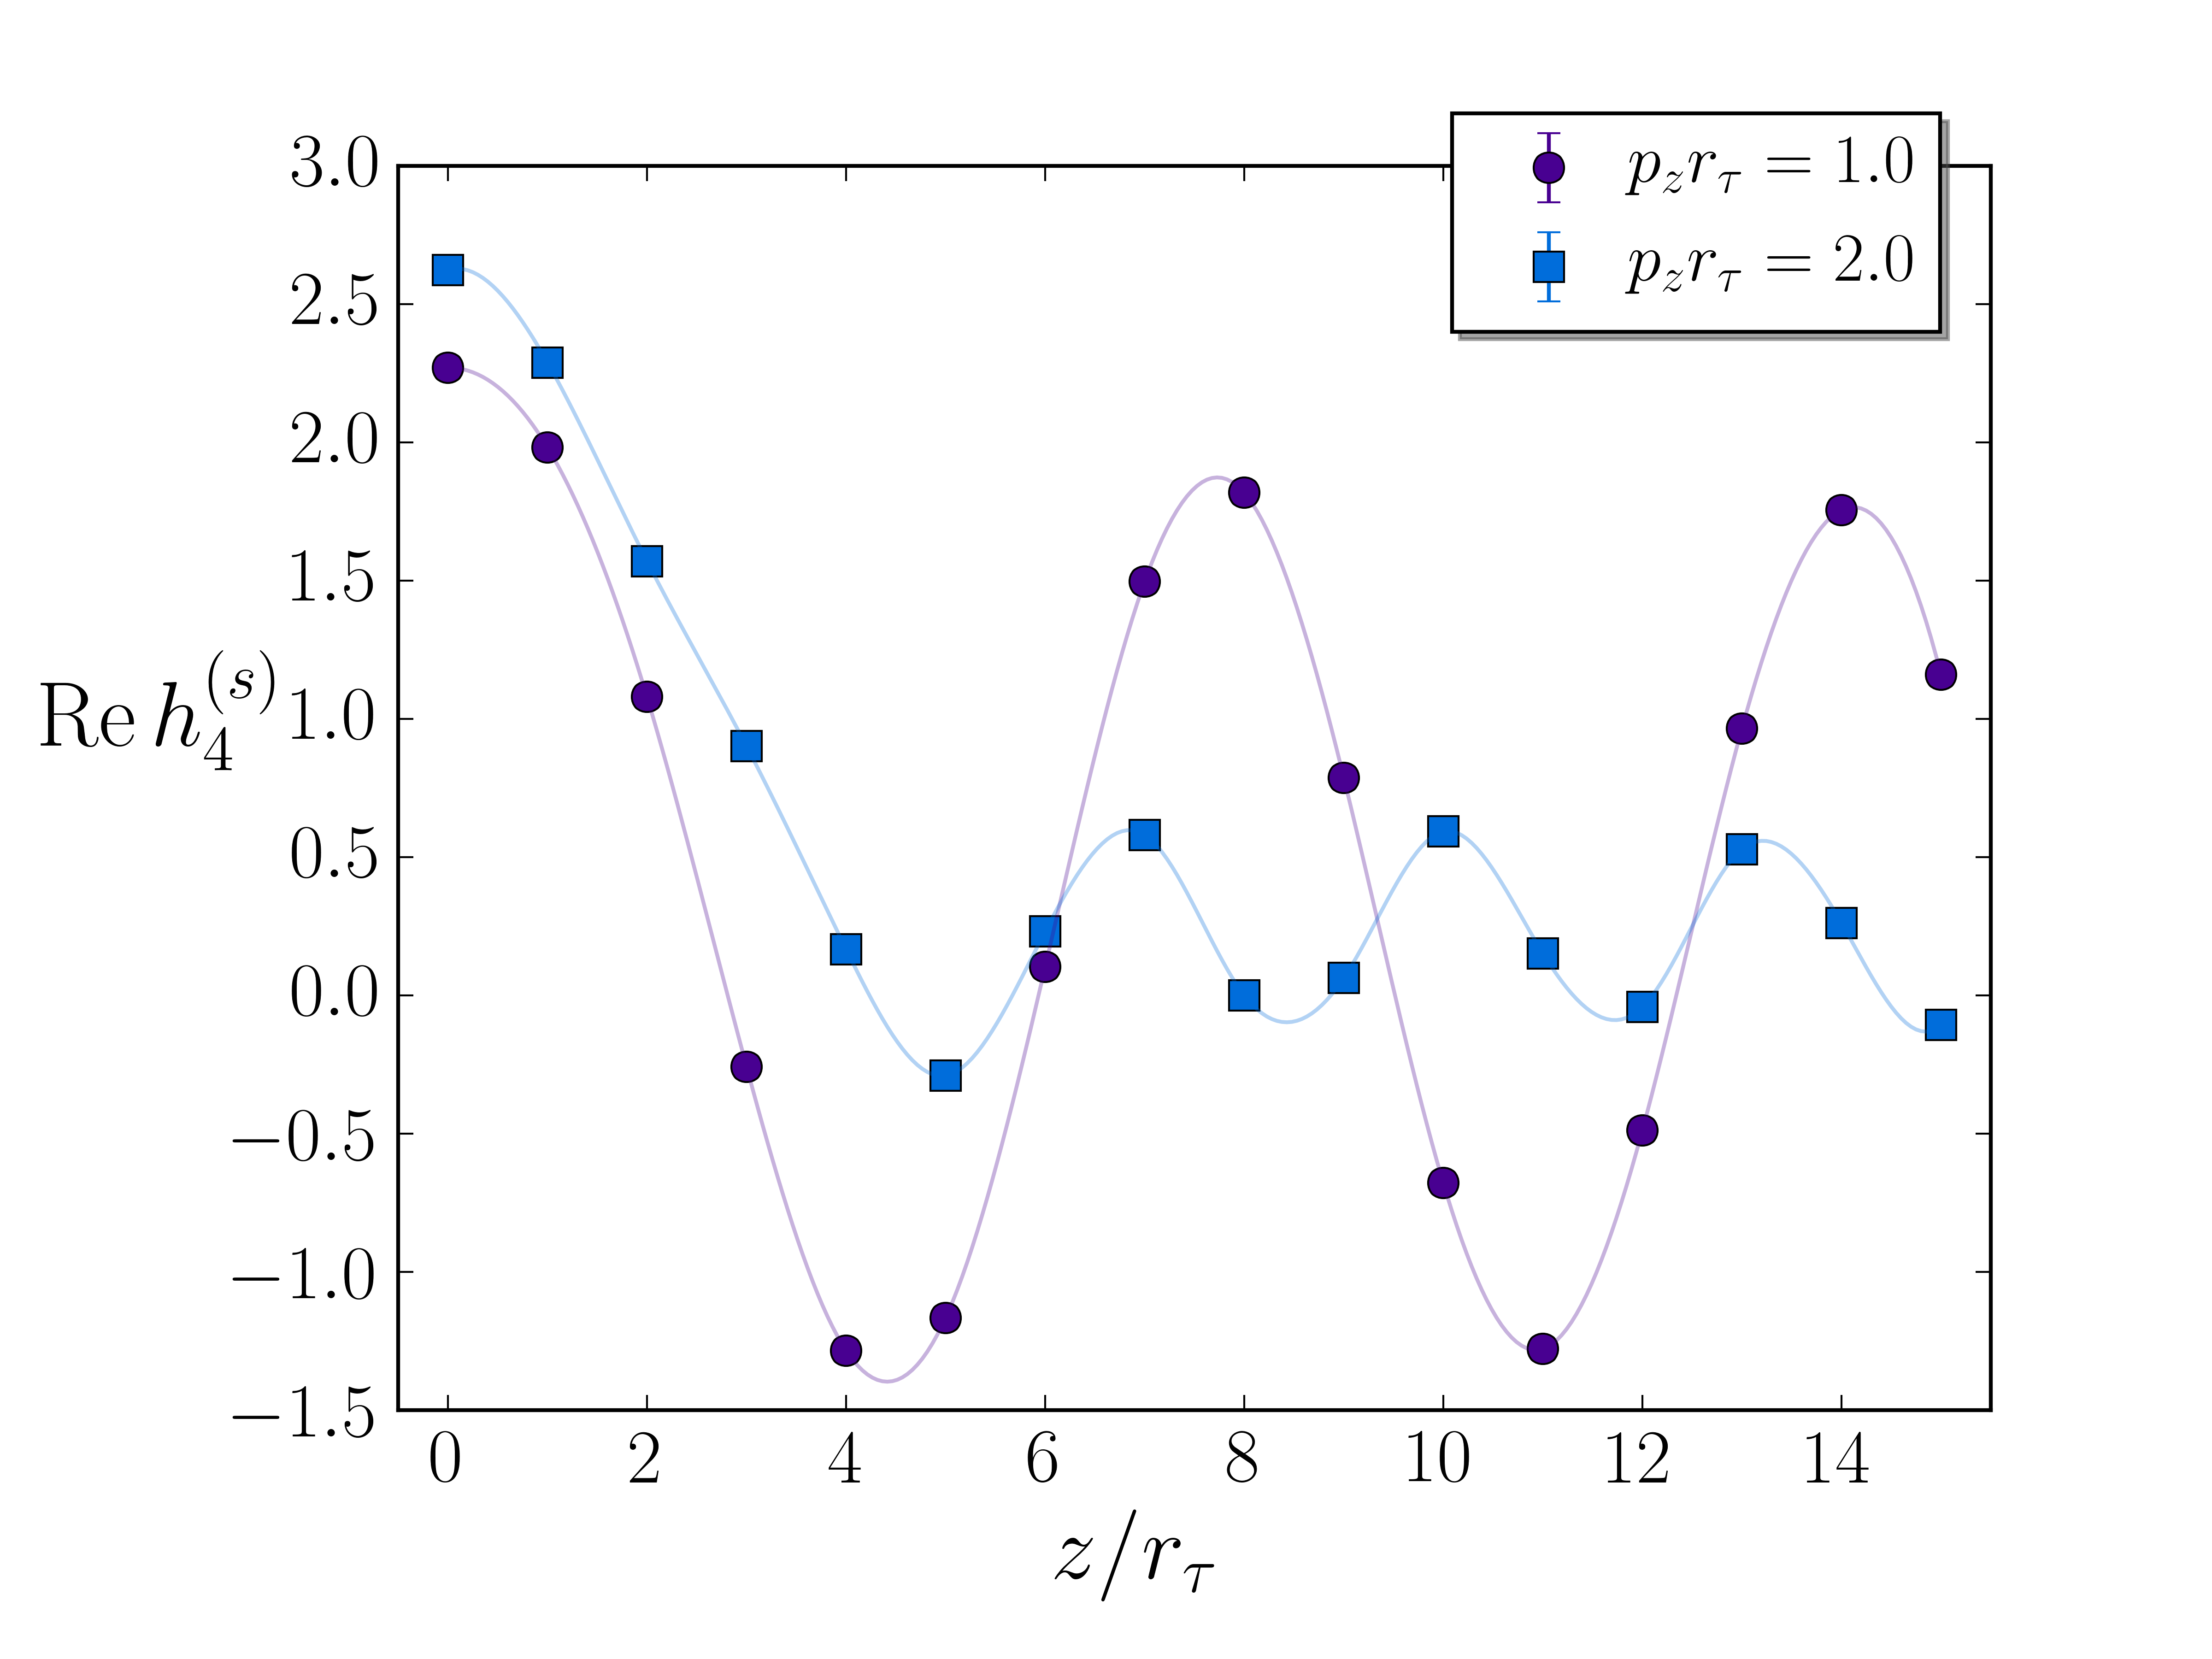
\includegraphics[width=0.4\textwidth,keepaspectratio]{images/hfn_re.png}\\
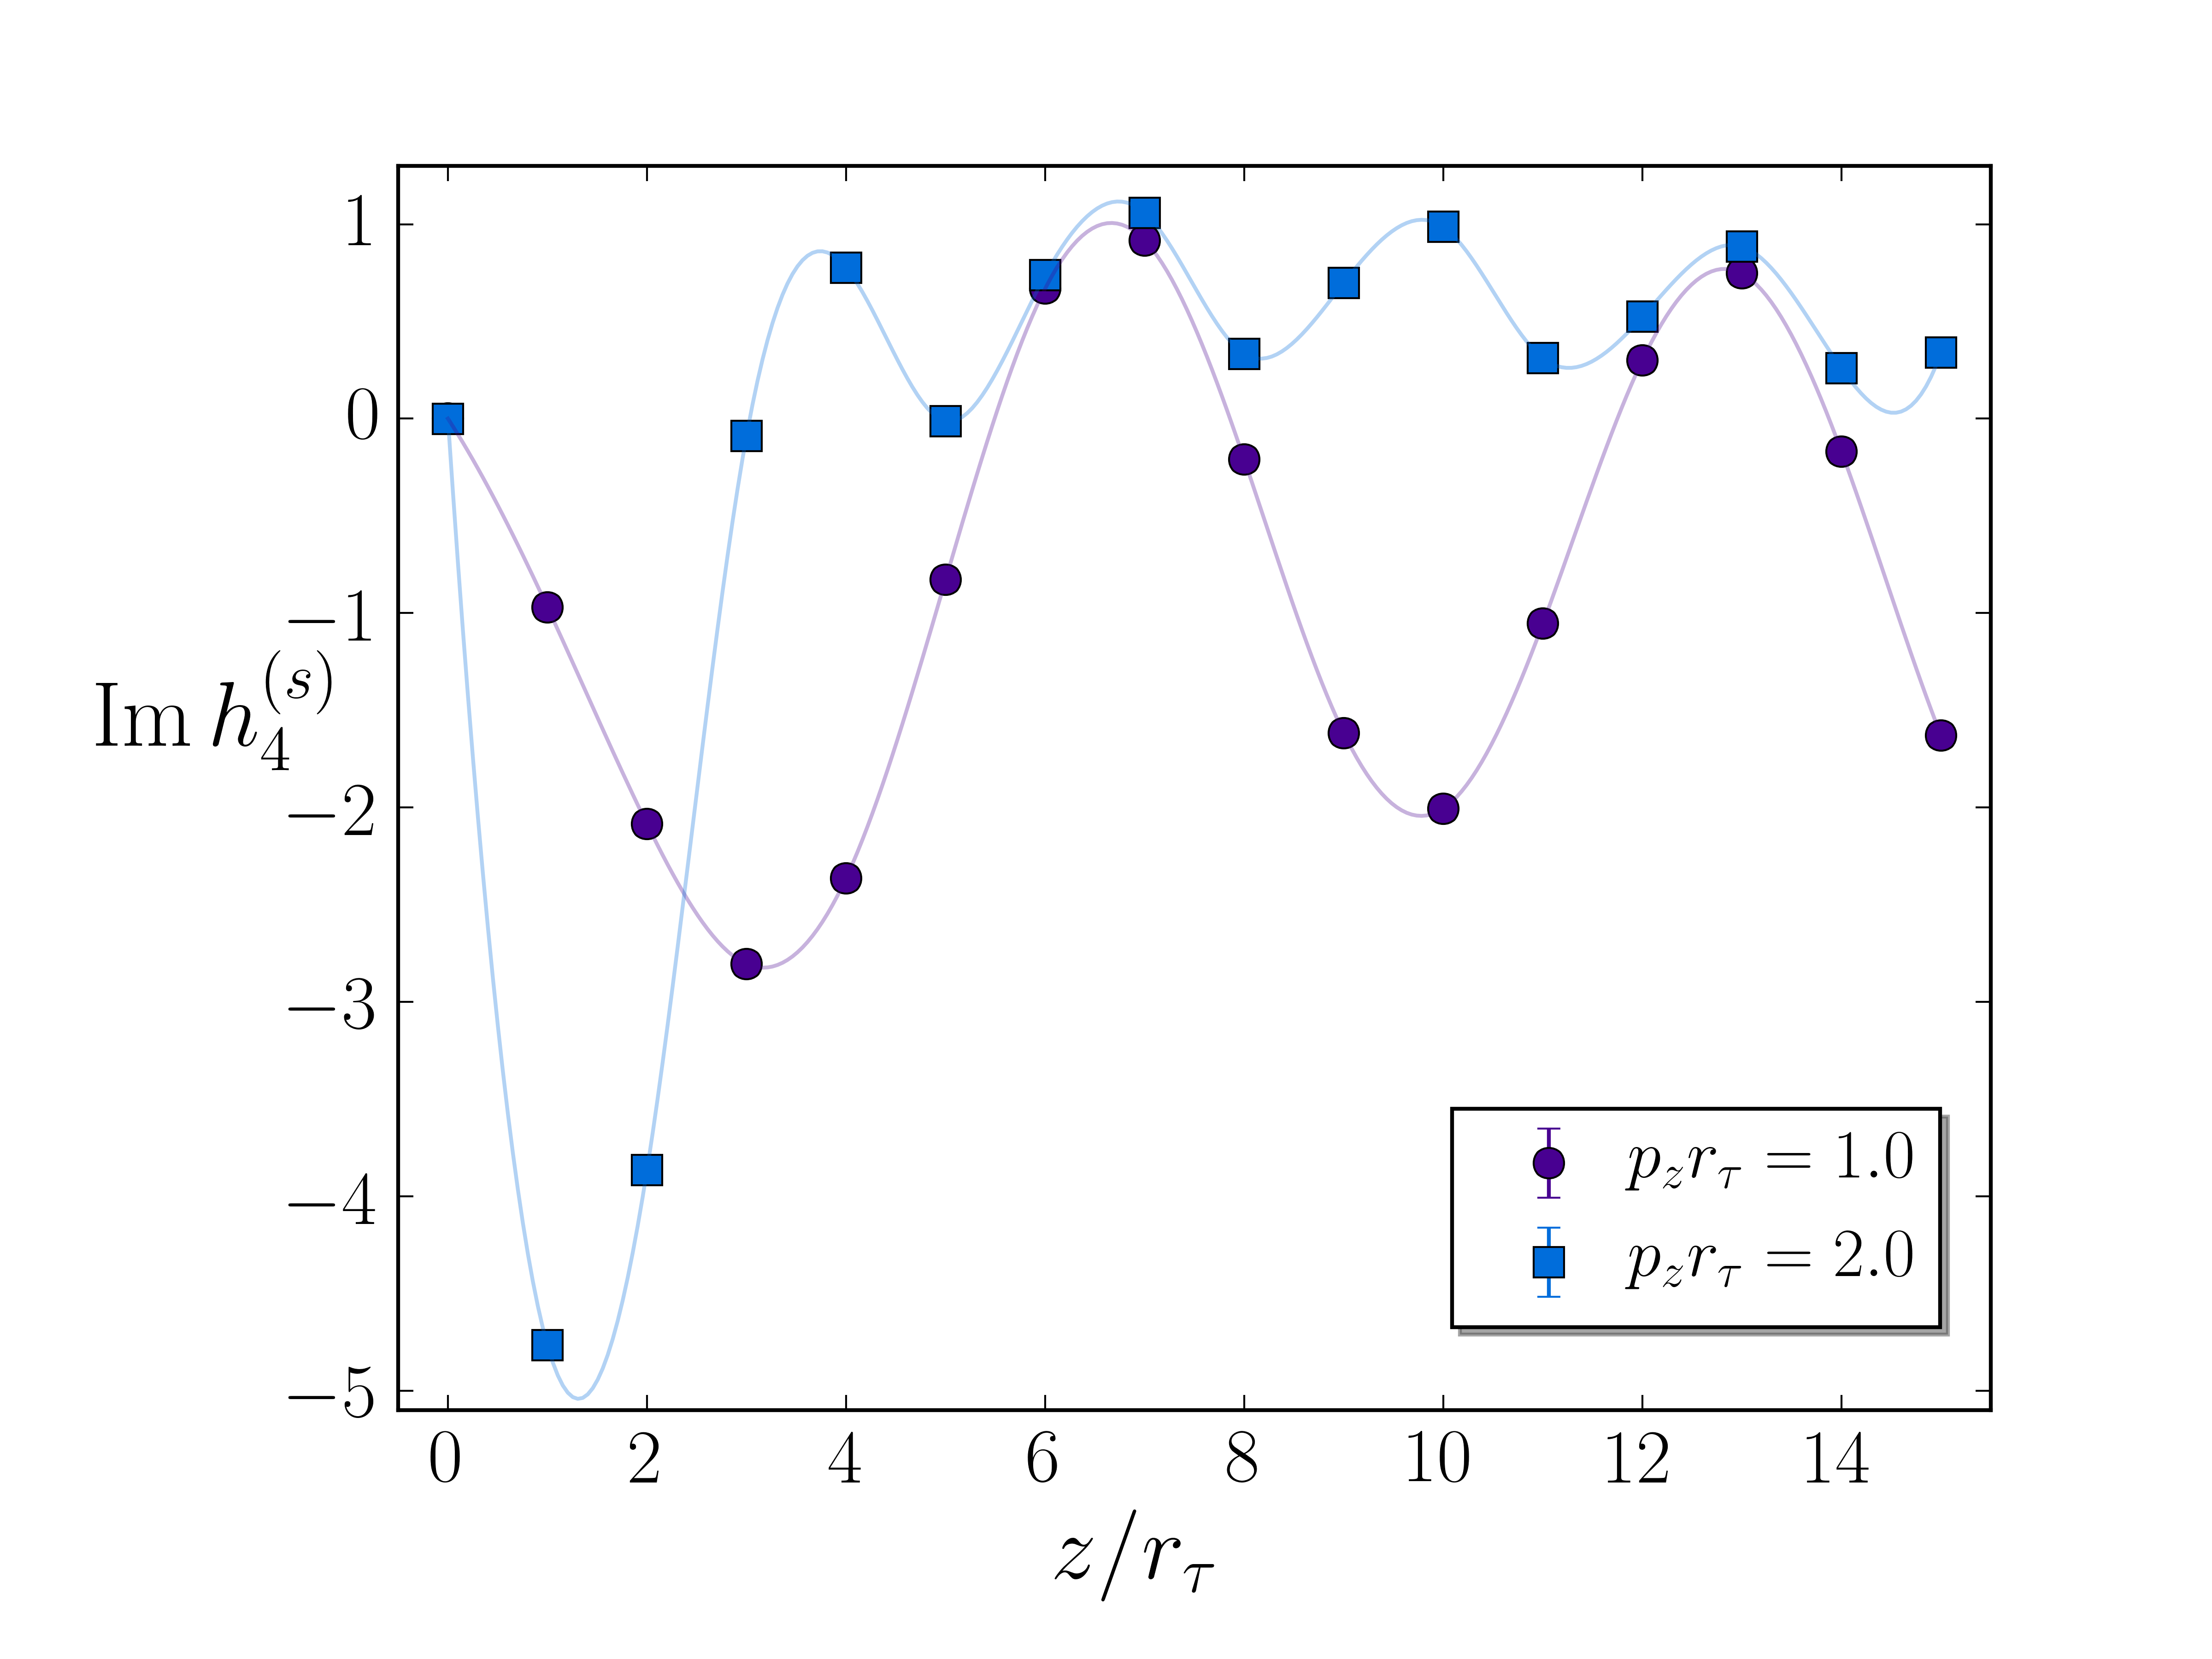
\includegraphics[width=0.4\textwidth,keepaspectratio]{images/hfn_im.png}
\end{figure}
